\documentclass[11pt,letterpaper]{article}

\usepackage[utf8]{inputenc}
\usepackage[T1]{fontenc}
\usepackage[spanish,es-nodecimaldot]{babel}
\usepackage{amsmath,amssymb,amsfonts}
\usepackage{booktabs}
\usepackage{array}
\usepackage{graphicx}
\usepackage{float}
\usepackage{geometry}
\usepackage{xcolor}
\usepackage{hyperref}
\usepackage{caption}
\usepackage{subcaption}

\geometry{margin=2.4cm}
\graphicspath{{outputs_sbm/}}

\hypersetup{
    colorlinks=true,
    linkcolor=blue!45!black,
    urlcolor=blue!45!black,
    citecolor=blue!45!black
}

\title{Caso de estudio: inferencia estadistica de comunidades en una red S\&P 500}
\author{LDS1121 - Redes complejas}
\date{}

\newcommand{\Gmini}{G_{\mathrm{mini}}}
\newcommand{\EE}{\mathbb{E}}

\begin{document}

\maketitle

\begin{abstract}
Este documento interpreta los resultados obtenidos al ajustar un modelo de bloques estocasticos corregido por grado a una red de relaciones proveedor/comprador entre empresas del S\&P 500. La notacion sigue el apunte \emph{Metodos basados en inferencia estadistica}: los grupos son $1,\ldots,q$, la asignacion latente es $g=(g_1,\ldots,g_n)$, los parametros de grado esperado son $c_i$, y la matriz de intensidades comunitarias es $\Omega=(\omega_{rs})$. El resultado principal es que el criterio penalizado selecciona $q=3$ tanto en la red completa como en la minired. La particion no representa solo comunidades densas: separa un bloque asortativo de consumo/pagos/retail y una estructura tecnologica disasortativa, en la cual dos bloques se conectan intensamente entre si.
\end{abstract}

\section{Planteamiento del caso}

La red original es dirigida: una arista $u\to v$ se interpreta como una relacion proveedor $\to$ comprador. Para el ajuste del modelo se usa la proyeccion no dirigida $G_1$, de modo que dos empresas quedan conectadas si existe al menos una relacion en cualquier direccion. Si $A^\rightarrow$ denota la matriz dirigida, la matriz usada en la inferencia es
\[
    A_{ij}=\mathbf{1}\{A^\rightarrow_{ij}+A^\rightarrow_{ji}>0\}.
\]

Esta transformacion conserva la existencia de relacion economica, pero no su direccion. Por tanto, las comunidades inferidas no deben leerse como cadenas causales de suministro, sino como patrones estructurales de asociacion.

Se analizan dos redes:
\[
    G_1=(V,E),\qquad
    \Gmini=G_1[V_{\mathrm{mini}}],
    \qquad
    V_{\mathrm{mini}}=\{i\in V:\; k_i\ge 2\}.
\]
La red completa tiene $30$ nodos, $37$ aristas y dos componentes conexas de tamanos $11$ y $19$. La minired tiene $15$ nodos, $22$ aristas y dos componentes conexas de tamanos $7$ y $8$. Esta separacion en componentes ya anticipa parte del resultado: el modelo no puede colocar aristas entre componentes desconectadas, por lo que la inferencia debe reflejar esa estructura.

\section{Modelo y notacion}

Seguimos la notacion del apunte. Sea $A$ la matriz de adyacencia no dirigida, con entradas $A_{ij}$. El grado observado del nodo $i$ es
\[
    k_i=\sum_j A_{ij},
    \qquad
    2m=\sum_i k_i.
\]
El modelo de bloques estocasticos corregido por grado divide los nodos en $q$ grupos etiquetados por $1,\ldots,q$. La etiqueta del nodo $i$ es $g_i$. Condicionalmente a $g$, el modelo coloca aristas con media proporcional a
\[
    \omega_{g_i g_j}\frac{c_i c_j}{2m}.
\]
Aqui $c_i$ captura la propension individual del nodo $i$ a tener aristas, mientras que $\omega_{rs}$ captura la intensidad de conexion entre los grupos $r$ y $s$.

Para una asignacion fija $g$, definimos
\[
    \kappa_r=\sum_i \delta_{g_i r}c_i,
    \qquad
    m_{rs}=\sum_{ij}\delta_{g_i r}\delta_{g_j s}A_{ij}.
\]
La cantidad $\kappa_r$ mide el volumen de grado esperado del grupo $r$, y $m_{rs}$ mide la masa observada de aristas entre los grupos $r$ y $s$. En redes no dirigidas, esta convencion cuenta dos veces la masa total, de modo que
\[
    \sum_{r,s}m_{rs}=2m.
\]

Al maximizar la log-verosimilitud con respecto a los parametros continuos, se obtienen los estimadores
\[
    \hat c_i=k_i,
    \qquad
    \hat\omega_{rs}
    =
    \frac{2m\,m_{rs}}{\kappa_r\kappa_s}.
\]
Sustituyendo estos estimadores se obtiene la log-verosimilitud perfilada
\[
    L(g)
    =
    \frac{1}{2}\sum_{r,s}m_{rs}
    \log\left(\frac{m_{rs}}{\kappa_r\kappa_s}\right)
    +\text{constantes}.
\]
El problema de deteccion de comunidades es entonces
\[
    \hat g_q=\arg\max_{g:V\to\{1,\ldots,q\}} L(g).
\]

\subsection{Como se interpreta \texorpdfstring{$\hat\omega_{rs}$}{omega rs}}

La formula
\[
    \hat\omega_{rs}
    =
    \frac{2m\,m_{rs}}{\kappa_r\kappa_s}
\]
es el centro interpretativo del caso. Si dos grupos tienen mucho volumen de grado, entonces $\kappa_r\kappa_s$ es grande y el modelo espera cierta cantidad de aristas entre ellos aun sin estructura especial. Por eso $\hat\omega_{rs}$ no mide solamente cuantas aristas hay; mide cuantas hay \emph{en relacion con lo que se esperaria por grado}.

Una diagonal grande, $\hat\omega_{rr}$, indica estructura asortativa: los nodos del grupo $r$ se conectan entre si mas de lo esperado. Una entrada fuera de la diagonal grande, $\hat\omega_{rs}$ con $r\ne s$, indica estructura disasortativa o de roles: los nodos de $r$ se conectan preferentemente con los de $s$.

\section{Seleccion del numero de grupos}

Para cada valor de $q$ se maximizo $L(g)$ mediante busqueda greedy con multiples arranques. Como $L(g)$ tiende a mejorar al aumentar $q$, se uso tambien una penalizacion tipo BIC:
\[
    \operatorname{BIC}_{\mathrm{like}}(q)
    =
    -2\hat L_q+p_q\log(2m),
    \qquad
    p_q\approx \frac{q(q+1)}{2}-q.
\]
El menor valor del criterio penalizado se obtuvo en $q=3$ para ambas redes.

\begin{table}[H]
\centering
\caption{Barrido de $q$ para la red completa y la minired. Menor BIC-like es mejor.}
\begin{tabular}{llrrr}
\toprule
Red & $q$ & $L$ perfilada & BIC-like & Modularidad diagnostica\\
\midrule
$G_1$ & 2 & -135.264 & 274.832 & 0.456\\
$G_1$ & 3 & -118.629 & \textbf{250.169} & 0.018\\
$G_1$ & 4 & -112.527 & 250.878 & -0.245\\
$G_1$ & 5 & -110.734 & 264.508 & -0.043\\
\midrule
$\Gmini$ & 2 & -68.369 & 140.521 & 0.483\\
$\Gmini$ & 3 & -59.358 & \textbf{130.068} & 0.067\\
$\Gmini$ & 4 & -55.677 & 134.059 & -0.214\\
$\Gmini$ & 5 & -54.519 & 146.879 & -0.143\\
\bottomrule
\end{tabular}
\end{table}

La modularidad es alta para $q=2$, pero no es el criterio que se esta optimizando. Esto no es una contradiccion: la modularidad favorece particiones asortativas, mientras que el DC-SBM puede detectar estructuras disasortativas. En este caso, $q=3$ permite separar una comunidad cerrada de consumo/pagos y, al mismo tiempo, dividir la parte tecnologica en dos roles complementarios.

\begin{figure}[H]
\centering
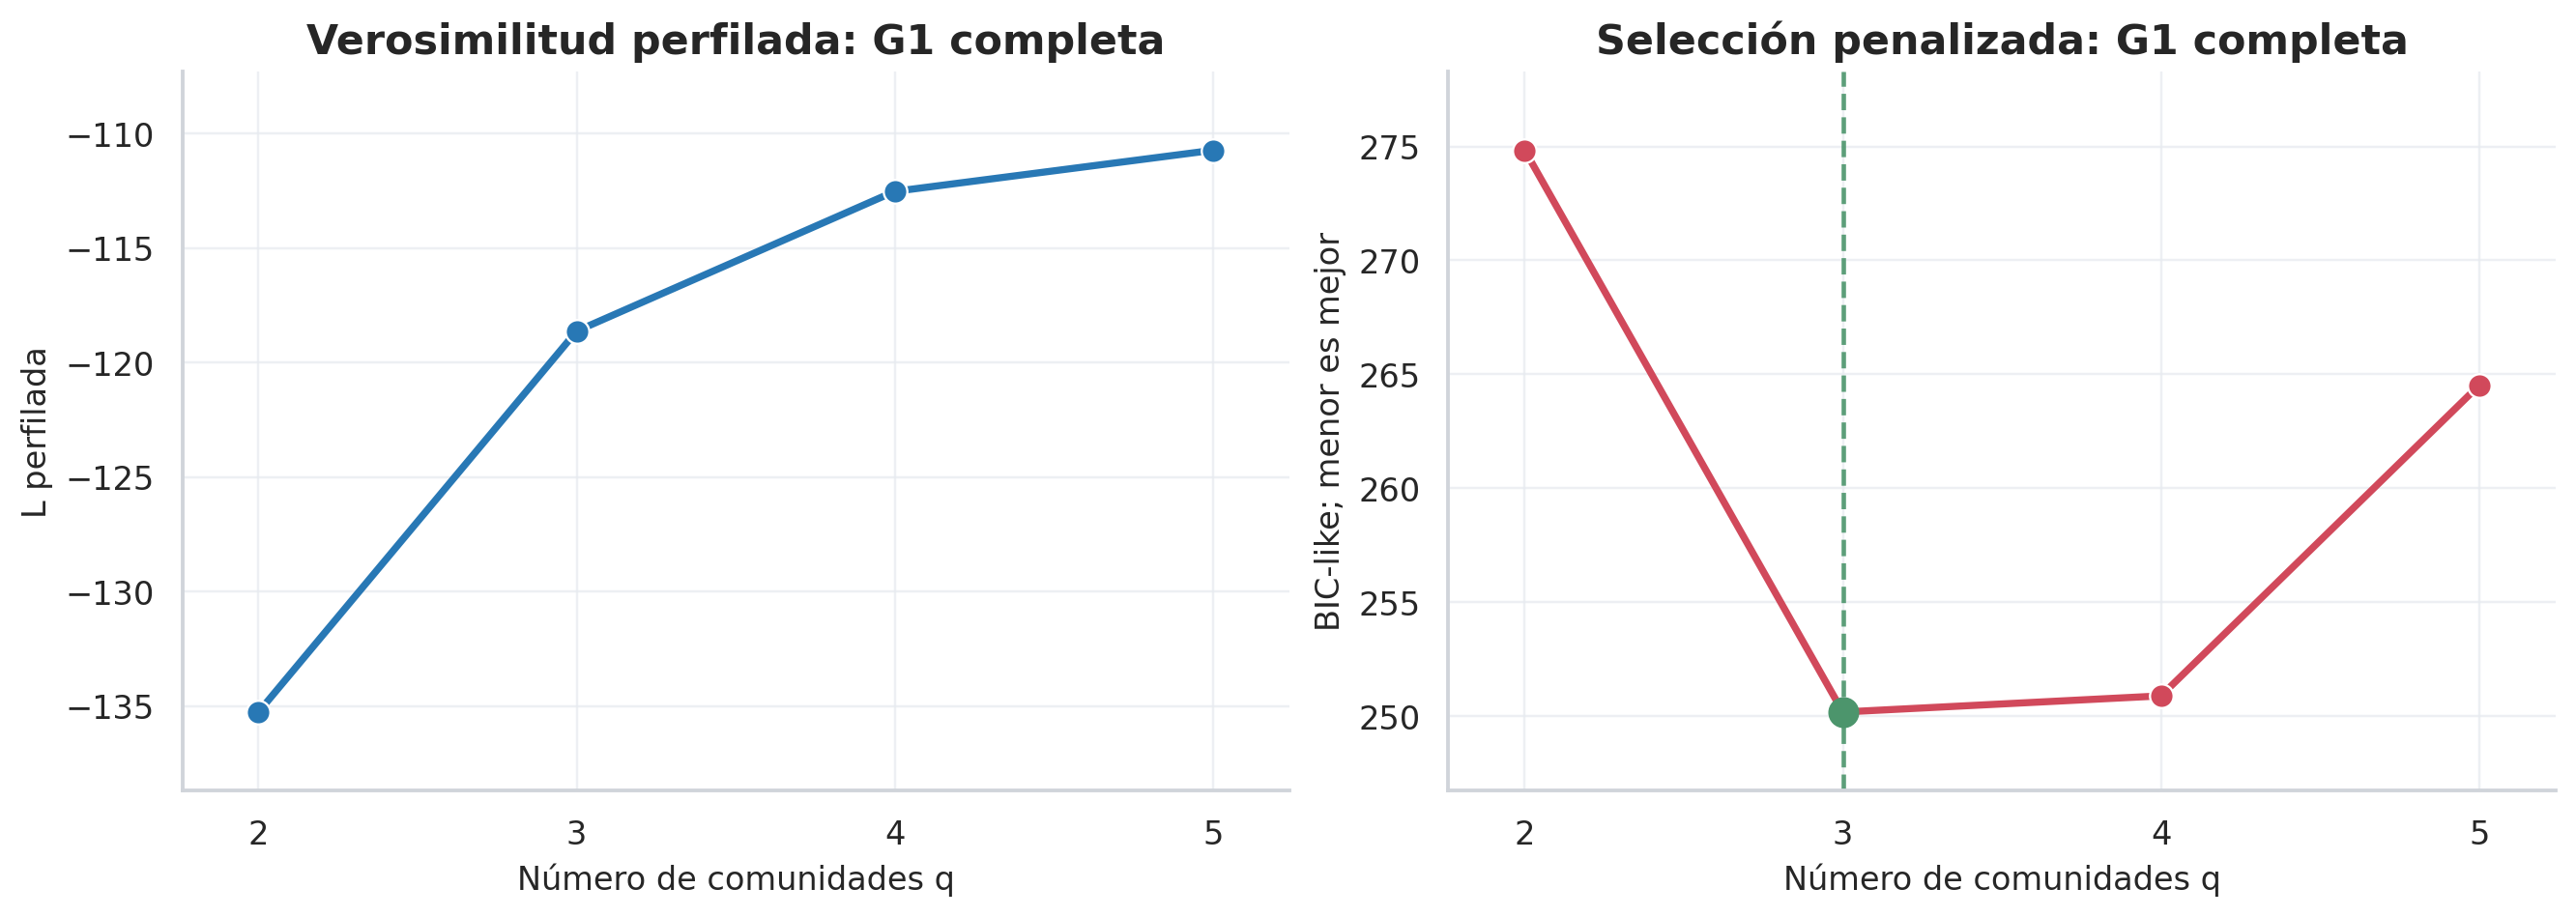
\includegraphics[width=0.82\linewidth]{barrido_q_G1_completa.png}
\caption{Barrido de $q$ para $G_1$. El criterio penalizado selecciona $q=3$.}
\end{figure}

\begin{figure}[H]
\centering
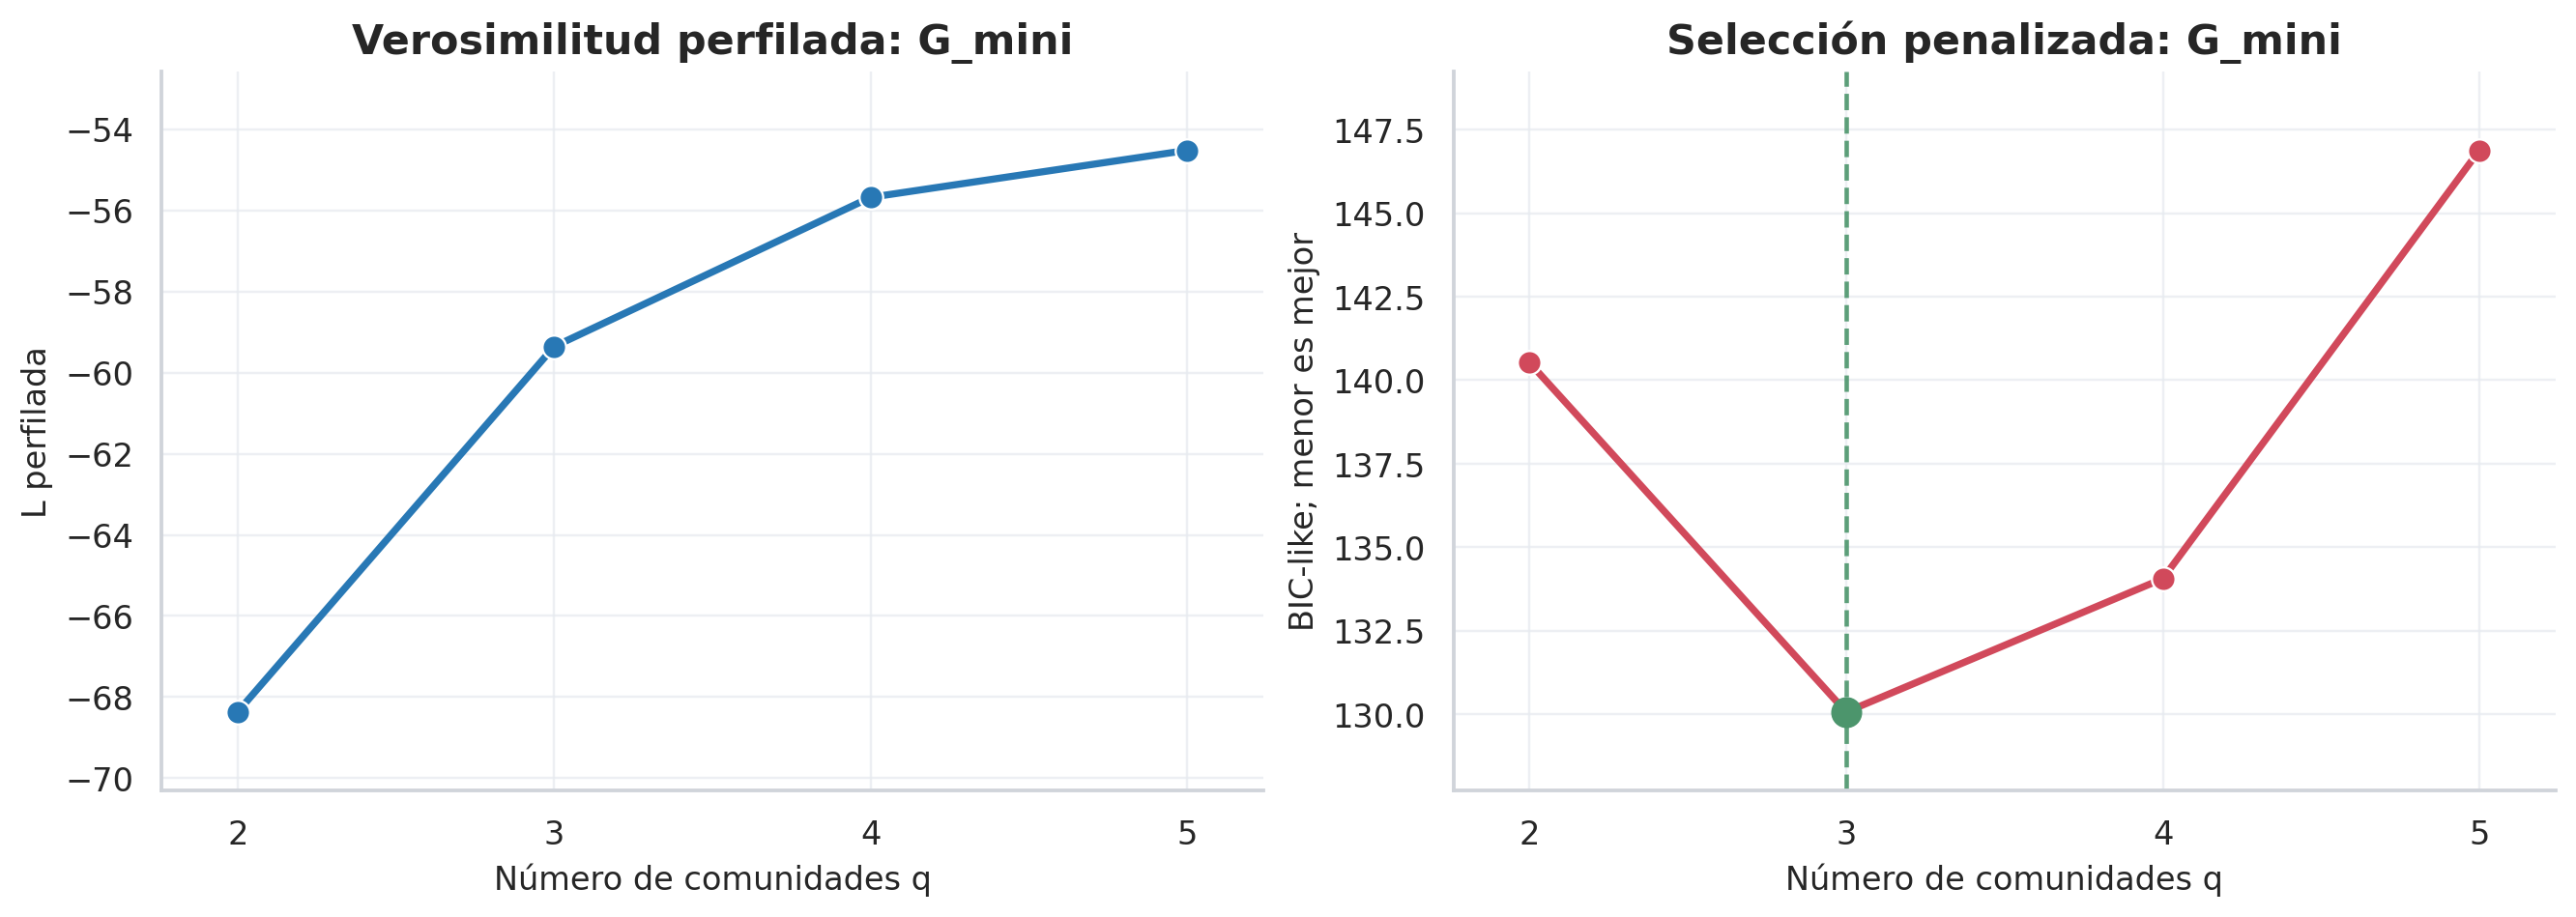
\includegraphics[width=0.82\linewidth]{barrido_q_G_mini.png}
\caption{Barrido de $q$ para $\Gmini$. La minired conserva la misma escala estructural: $q=3$.}
\end{figure}

\section{Resultados en la red completa}

En esta seccion usamos grupos $1,2,3$. La correspondencia con el notebook es:
\[
    C0\equiv 1,\qquad C1\equiv 2,\qquad C2\equiv 3.
\]
La particion estimada en $G_1$ es:

\begin{table}[H]
\centering
\caption{Comunidades estimadas en $G_1$.}
\resizebox{\textwidth}{!}{%
\begin{tabular}{clrrrp{7.2cm}}
\toprule
Grupo & Lectura & Nodos & Aristas internas & $\kappa_r$ & Miembros principales\\
\midrule
1 & Consumo, pagos y retail & 11 & 13 & 26 & AAPL, AVGO, BAC, BRK.B, COST, HD, JPM, MA, PG, V, WMT\\
2 & Infraestructura/IA y periferia conectada a plataformas & 11 & 0 & 24 & ABBV, AMD, CVX, GE, JNJ, LLY, NFLX, NVDA, PLTR, UNH, XOM\\
3 & Plataformas y compradores tecnologicos & 8 & 0 & 24 & AMZN, GOOG, GOOGL, META, MSFT, MU, ORCL, TSLA\\
\bottomrule
\end{tabular}
}
\end{table}

Las matrices agregadas por bloques fueron
\[
    M=
    \begin{pmatrix}
    26 & 0 & 0\\
    0 & 0 & 24\\
    0 & 24 & 0
    \end{pmatrix},
    \qquad
    \hat\Omega=
    \begin{pmatrix}
    2.846 & 0 & 0\\
    0 & 0 & 3.083\\
    0 & 3.083 & 0
    \end{pmatrix}.
\]

\subsection{Por que aparece un bloque cerrado de consumo/pagos}

El grupo $1$ tiene $\kappa_1=26$ y toda su masa observada queda en la diagonal: $m_{11}=26$. Como la red completa tiene $m=37$, entonces $2m=74$ y
\[
    \hat\omega_{11}
    =
    \frac{74\cdot 26}{26^2}
    =
    \frac{74}{26}
    =
    2.846.
\]
Este valor alto significa que el bloque de consumo/pagos tiene mas conexion interna de la esperada bajo un modelo que solo respeta grados. Sustantivamente, esto refleja un subecosistema alrededor de `AAPL', pagos (`MA', `V'), retail (`WMT', `COST', `HD') y nodos financieros asociados (`BAC', `JPM', `BRK.B').

El hecho de que $m_{12}=m_{13}=0$ tambien es informativo. No solo se detecta una comunidad densa; se detecta una componente desconectada del bloque tecnologico. Por eso el grupo $1$ aparece como una comunidad asortativa limpia.

\subsection{Por que la parte tecnologica se parte en dos roles}

Los grupos $2$ y $3$ tienen $\kappa_2=\kappa_3=24$, pero no tienen aristas internas:
\[
    m_{22}=m_{33}=0.
\]
Toda su masa va de un grupo al otro:
\[
    m_{23}=m_{32}=24.
\]
Por tanto,
\[
    \hat\omega_{23}
    =
    \frac{74\cdot 24}{24\cdot 24}
    =
    \frac{74}{24}
    =
    3.083.
\]
Esta es la intensidad mas grande en $G_1$. Matematicamente, el modelo prefiere separar esta componente en dos bloques porque si se colocaran todos estos nodos en un solo grupo, el modelo describiria la region tecnologica como una comunidad densa. Pero los datos no tienen muchas aristas dentro de cada lado; tienen aristas cruzadas. La particion en dos roles aumenta la verosimilitud porque concentra masa en $m_{23}$ y $m_{32}$, y evita asignar probabilidad a diagonales que en realidad son cero.

La interpretacion economica es natural: un lado contiene nodos de infraestructura, semiconductores, IA y periferia conectada a plataformas (`NVDA', `AMD', `PLTR' y empresas conectadas a `AMZN' o `MSFT'); el otro contiene plataformas o compradores tecnologicos (`AMZN', `MSFT', `ORCL', `GOOGL', `TSLA'). La red no dice que todos los nodos tecnologicos sean parecidos; dice que hay una relacion de complementariedad entre dos lados.

\begin{figure}[H]
\centering
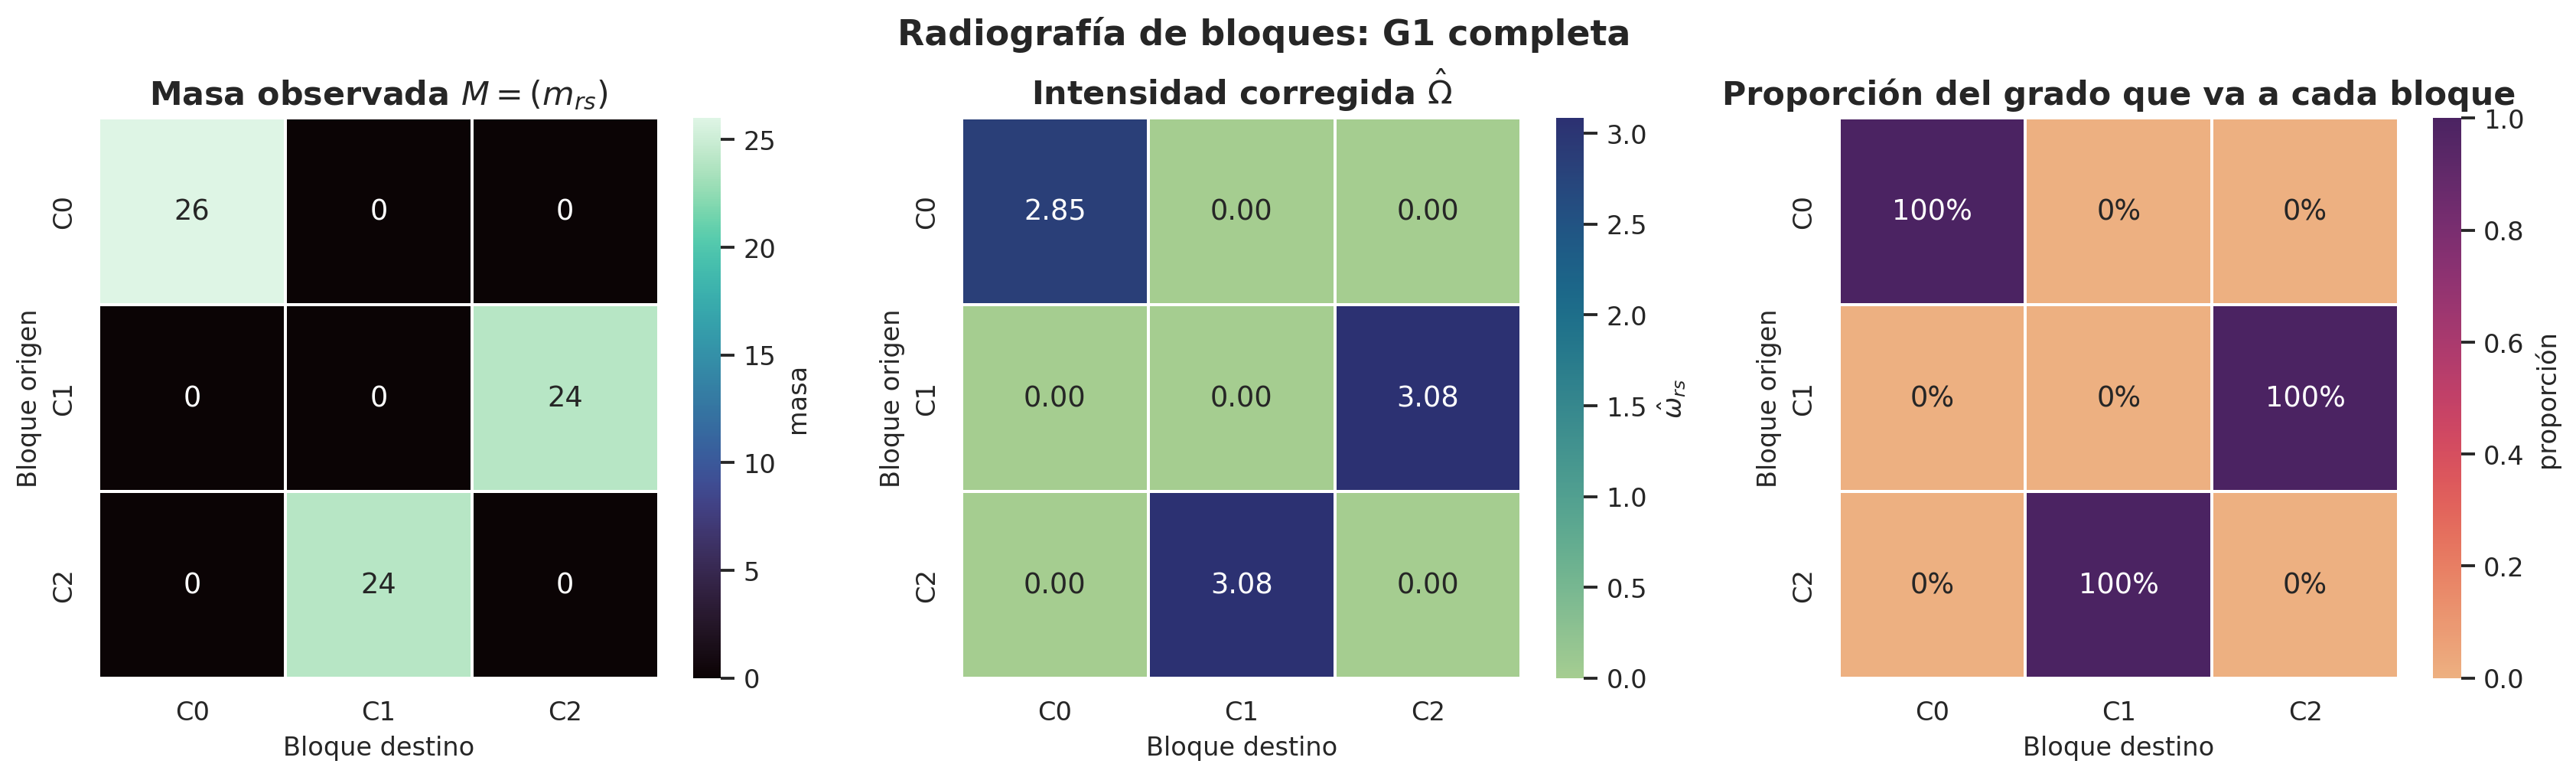
\includegraphics[width=0.95\linewidth]{radiografia_bloques_G1_completa.png}
\caption{Radiografia de bloques para $G_1$. La diagonal del grupo 1 muestra estructura asortativa; la masa entre los grupos 2 y 3 muestra estructura disasortativa.}
\end{figure}

\begin{figure}[H]
\centering
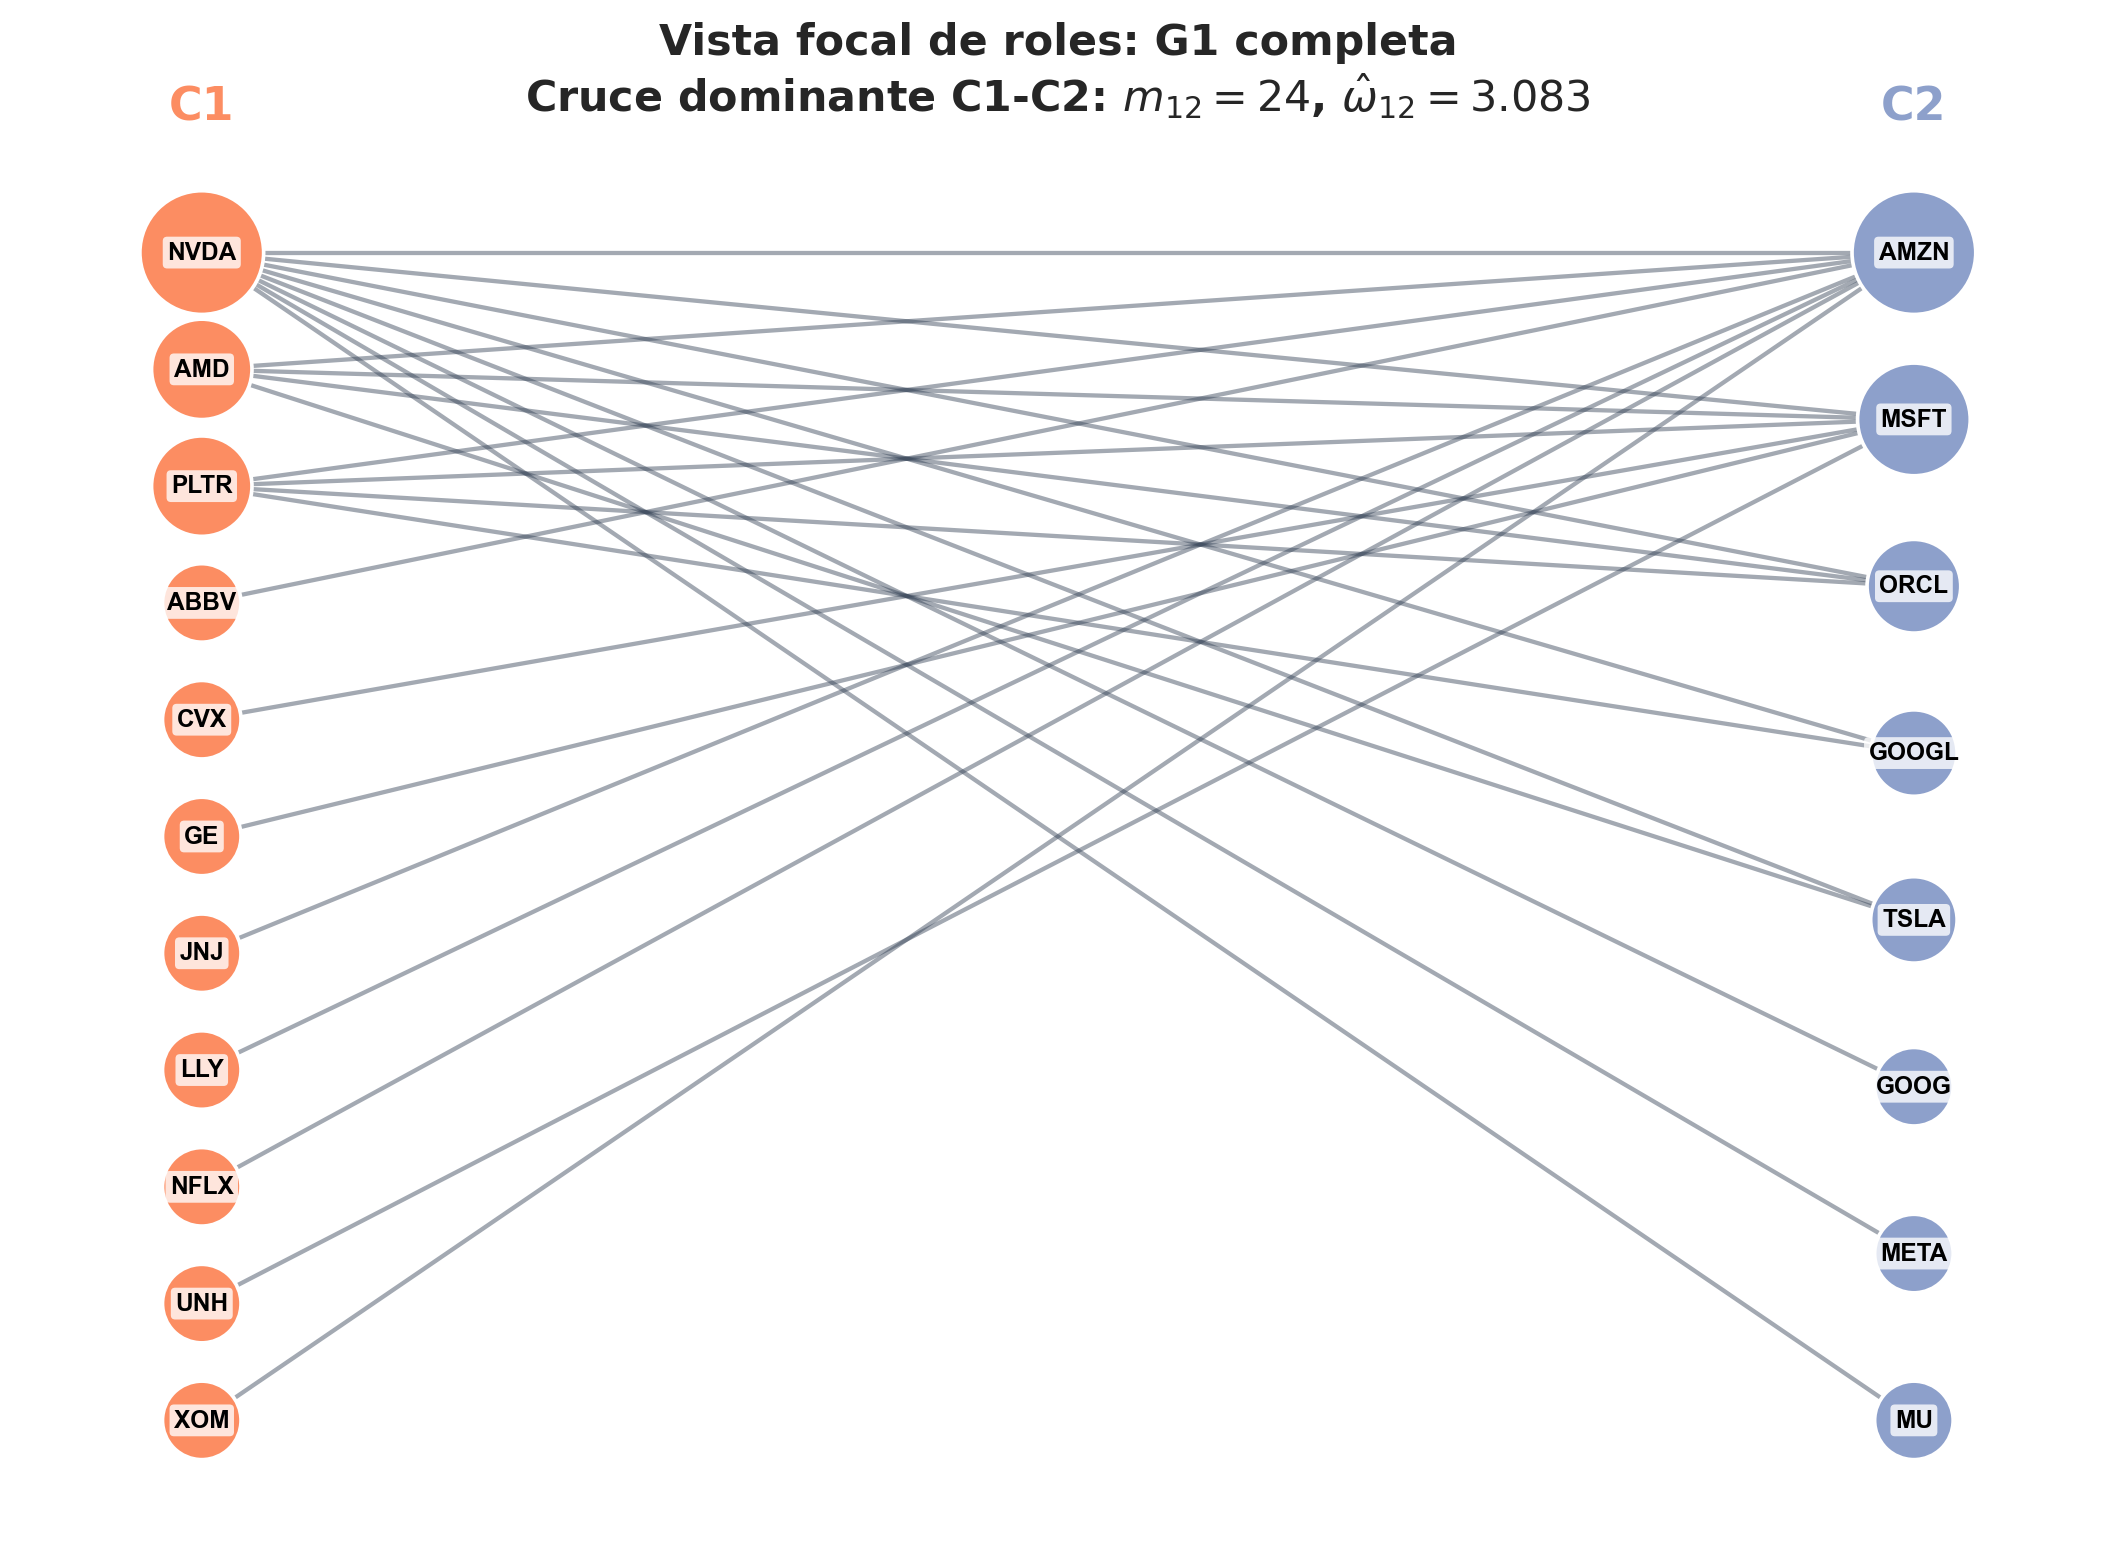
\includegraphics[width=0.95\linewidth]{vista_bipartita_dominante_G1_completa.png}
\caption{Vista focal del cruce dominante en $G_1$. El par de bloques 2--3 concentra la intensidad corregida mas alta.}
\end{figure}

\section{Resultados en la minired}

La minired elimina nodos de grado $1$ y conserva el nucleo relacional. La correspondencia de etiquetas vuelve a ser:
\[
    C0\equiv 1,\qquad C1\equiv 2,\qquad C2\equiv 3.
\]
La particion resultante fue:

\begin{table}[H]
\centering
\caption{Comunidades estimadas en $\Gmini$.}
\resizebox{\textwidth}{!}{%
\begin{tabular}{clrrrp{6.7cm}}
\toprule
Grupo & Lectura & Nodos & Aristas internas & $\kappa_r$ & Miembros\\
\midrule
1 & Nucleo pagos/retail & 7 & 9 & 18 & AAPL, BAC, COST, HD, MA, V, WMT\\
2 & Plataformas tecnologicas & 5 & 0 & 13 & AMZN, GOOGL, MSFT, ORCL, TSLA\\
3 & Infraestructura/IA & 3 & 0 & 13 & AMD, NVDA, PLTR\\
\bottomrule
\end{tabular}
}
\end{table}

Las matrices fueron
\[
    M=
    \begin{pmatrix}
    18 & 0 & 0\\
    0 & 0 & 13\\
    0 & 13 & 0
    \end{pmatrix},
    \qquad
    \hat\Omega=
    \begin{pmatrix}
    2.444 & 0 & 0\\
    0 & 0 & 3.385\\
    0 & 3.385 & 0
    \end{pmatrix}.
\]

Ahora $m=22$, por lo que $2m=44$. Para el bloque de pagos/retail,
\[
    \hat\omega_{11}
    =
    \frac{44\cdot 18}{18^2}
    =
    \frac{44}{18}
    =
    2.444.
\]
Para el cruce tecnologico,
\[
    \hat\omega_{23}
    =
    \frac{44\cdot 13}{13\cdot 13}
    =
    \frac{44}{13}
    =
    3.385.
\]
La intensidad cruzada aumenta al pasar a la minired. Esto ocurre porque se retiraron nodos hoja que aportaban contexto periferico, y quedo una estructura mas pura: plataformas tecnologicas en un lado e infraestructura/IA en el otro. La conclusion no cambia; se vuelve mas nitida.

\begin{figure}[H]
\centering
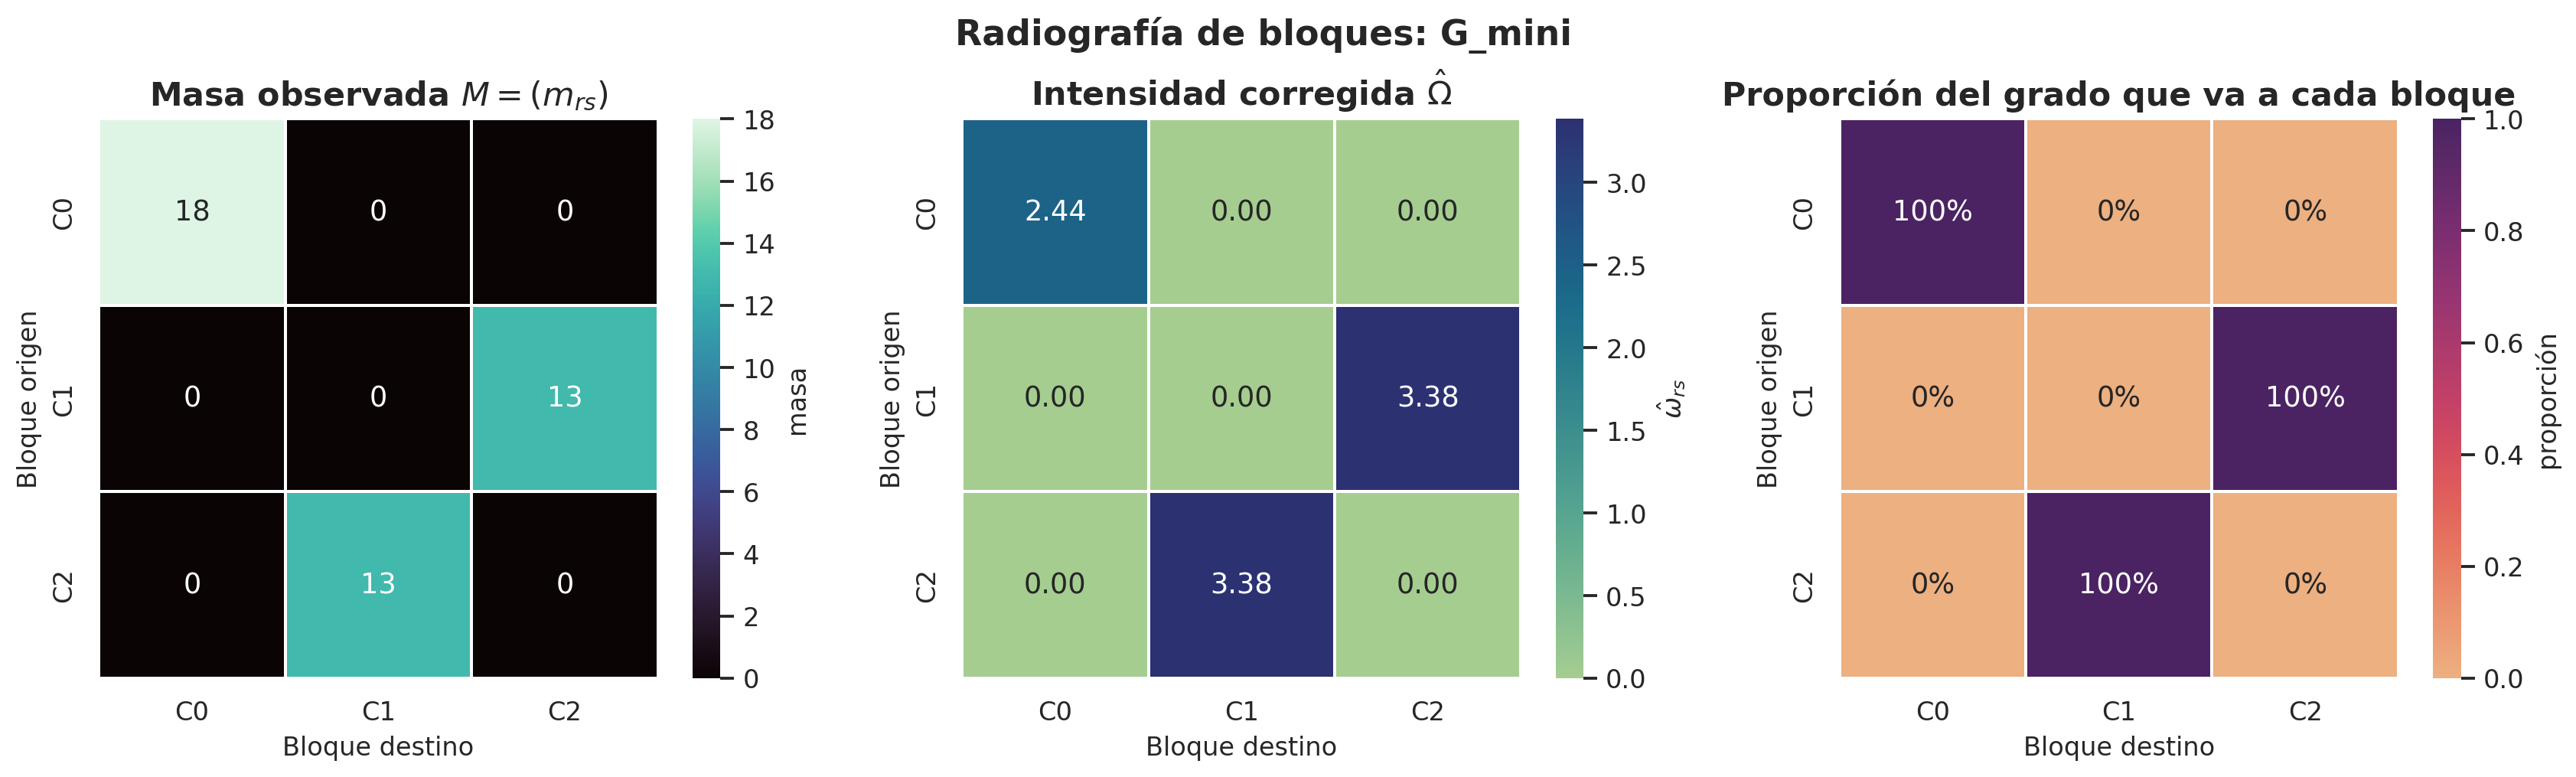
\includegraphics[width=0.95\linewidth]{radiografia_bloques_G_mini.png}
\caption{Radiografia de bloques para $\Gmini$. La estructura tecnologica disasortativa se vuelve mas clara al eliminar nodos hoja.}
\end{figure}

\begin{figure}[H]
\centering
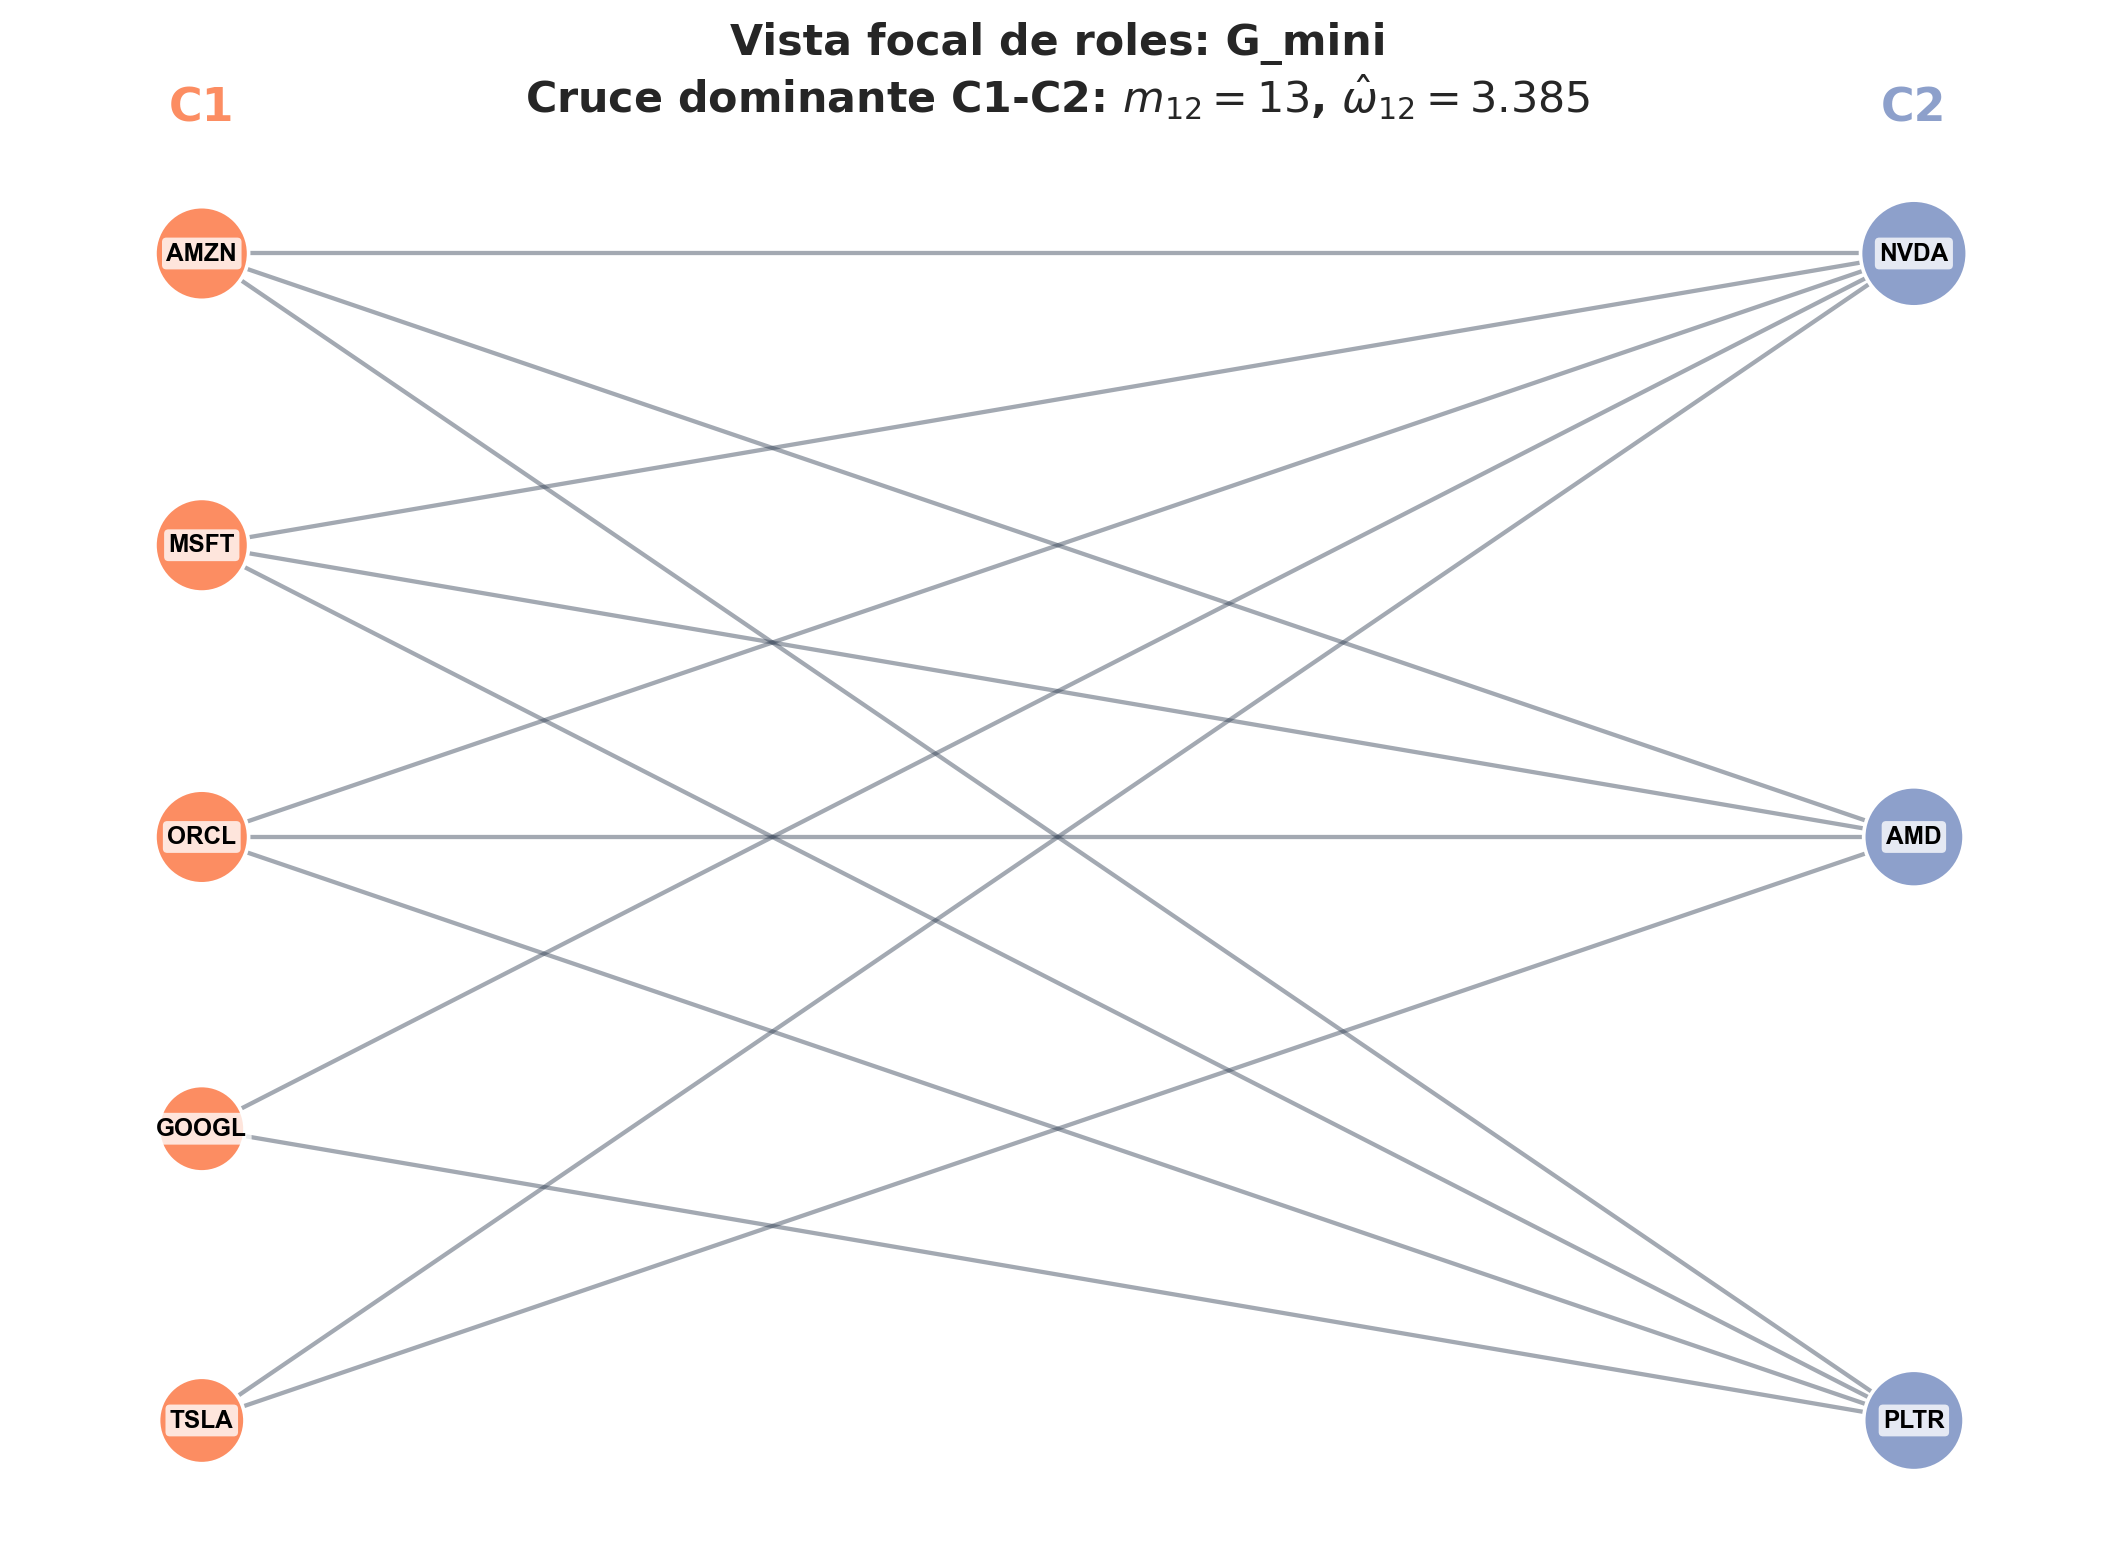
\includegraphics[width=0.95\linewidth]{vista_bipartita_dominante_G_mini.png}
\caption{Vista focal del cruce dominante en $\Gmini$. La relacion entre plataformas e infraestructura/IA concentra la mayor intensidad corregida.}
\end{figure}

\section{Lectura visual de las particiones}

Las figuras de adyacencia ordenada y red partida son utiles porque traducen las matrices $M$ y $\hat\Omega$ a patrones visuales.

\begin{figure}[H]
\centering
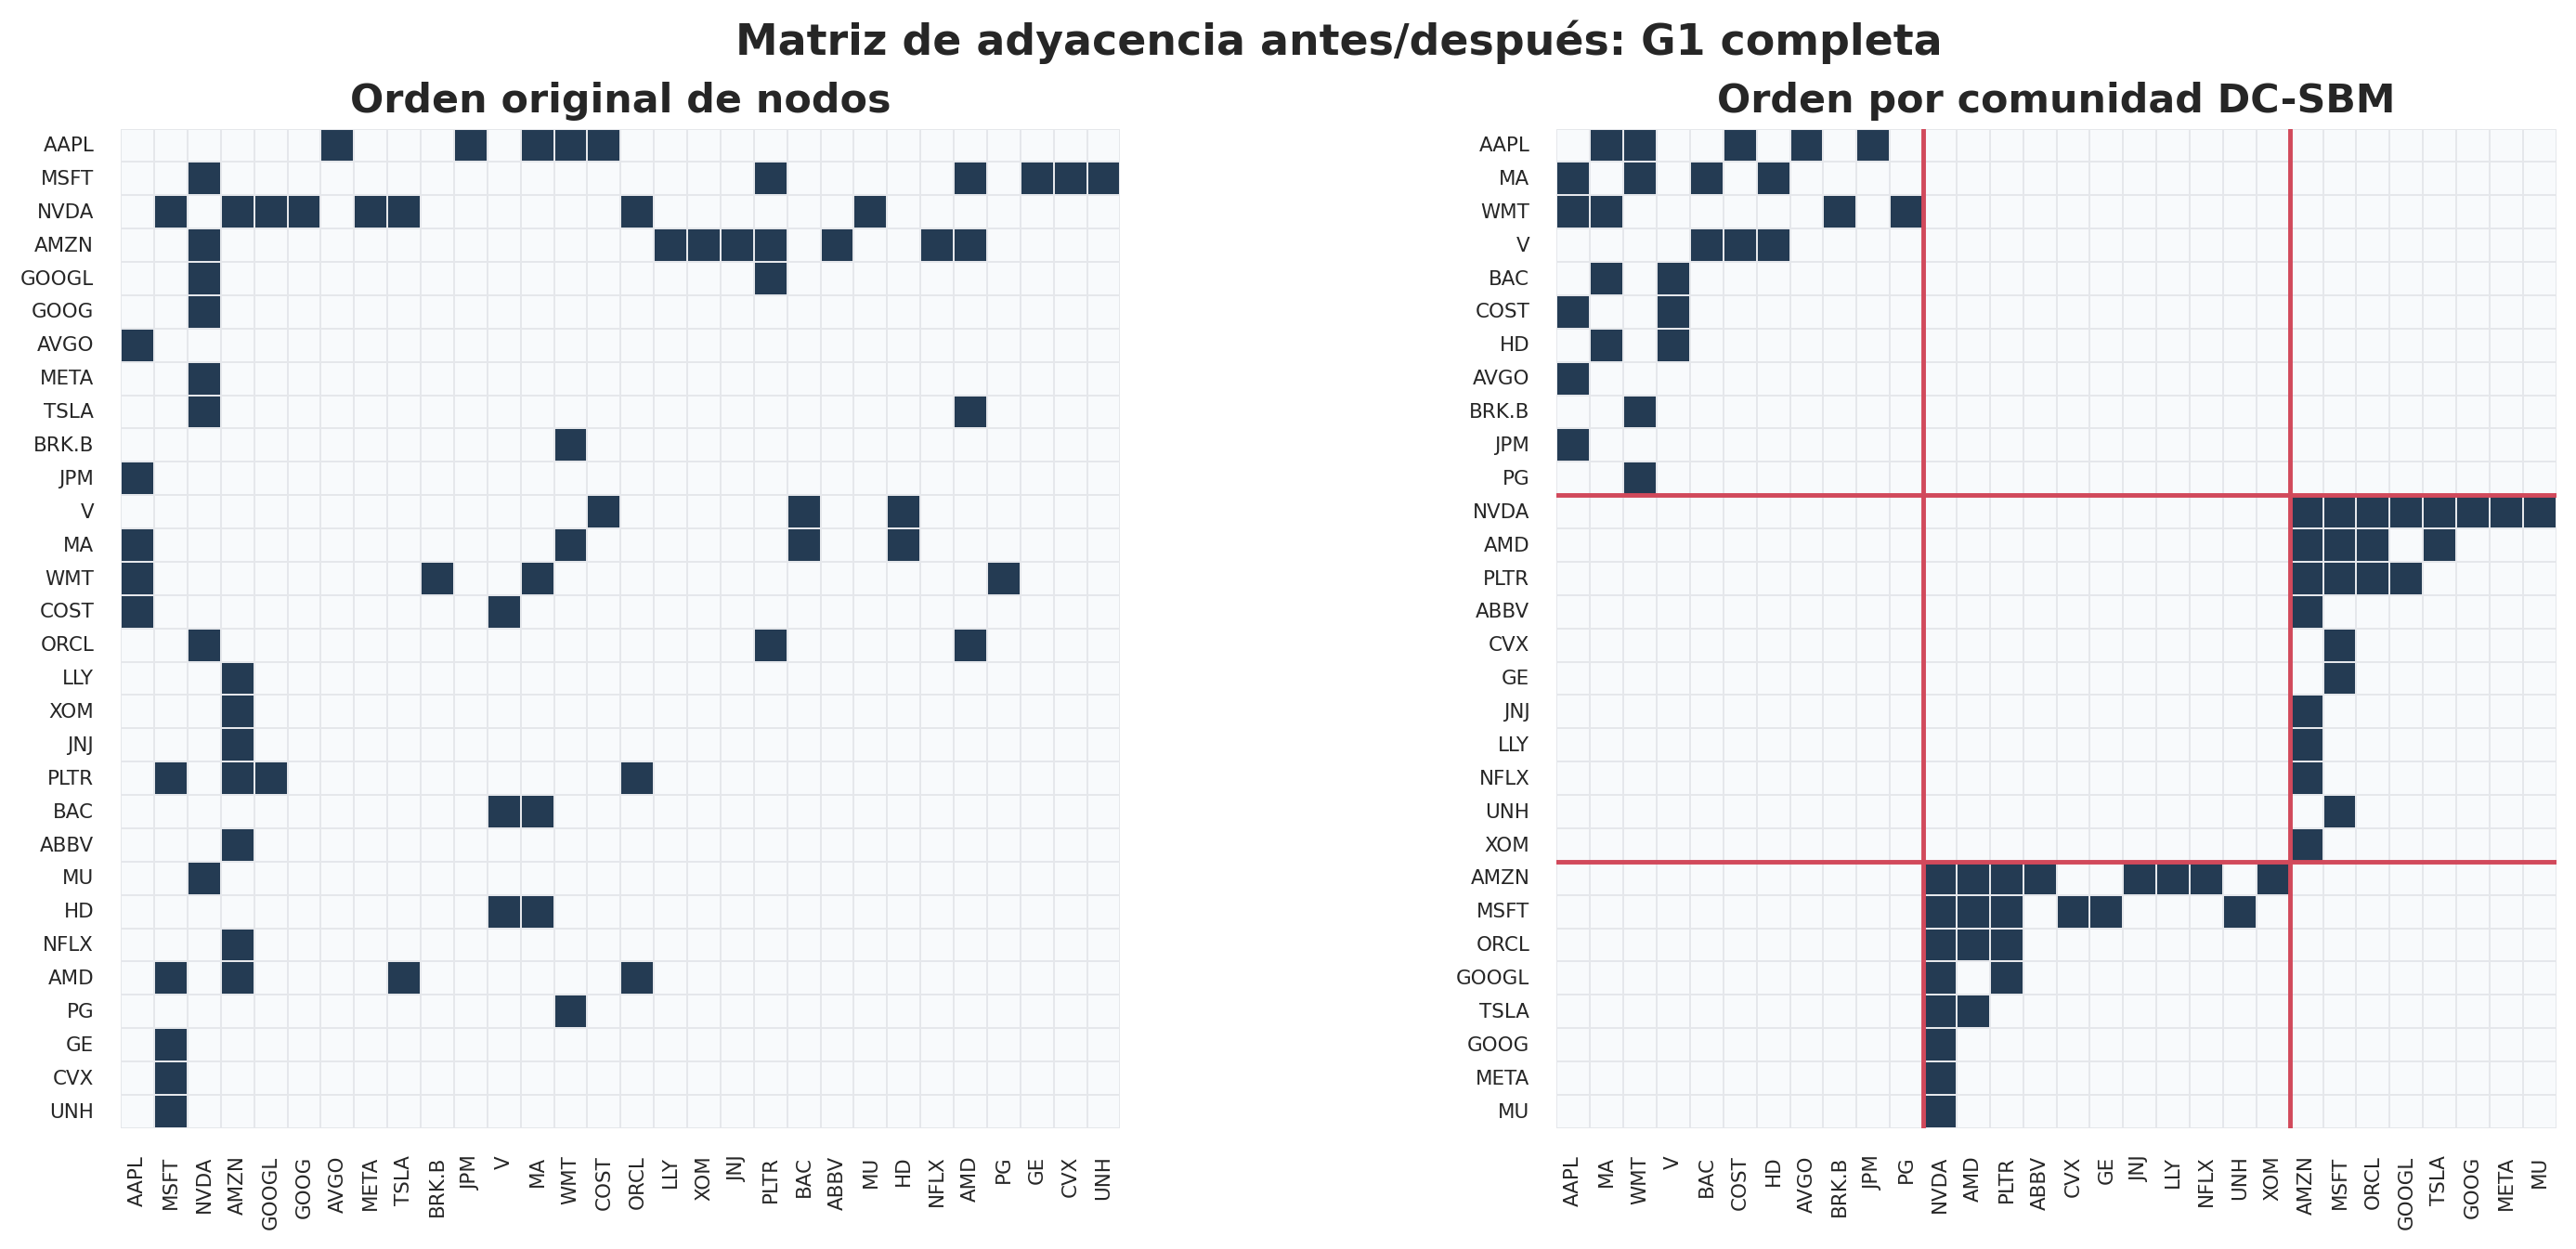
\includegraphics[width=0.95\linewidth]{adyacencia_antes_despues_G1_completa.png}
\caption{Matriz de adyacencia de $G_1$ antes y despues de ordenar por comunidades. La ordenacion revela un bloque diagonal para consumo/pagos y dos rectangulos fuera de la diagonal para la parte tecnologica.}
\end{figure}

\begin{figure}[H]
\centering
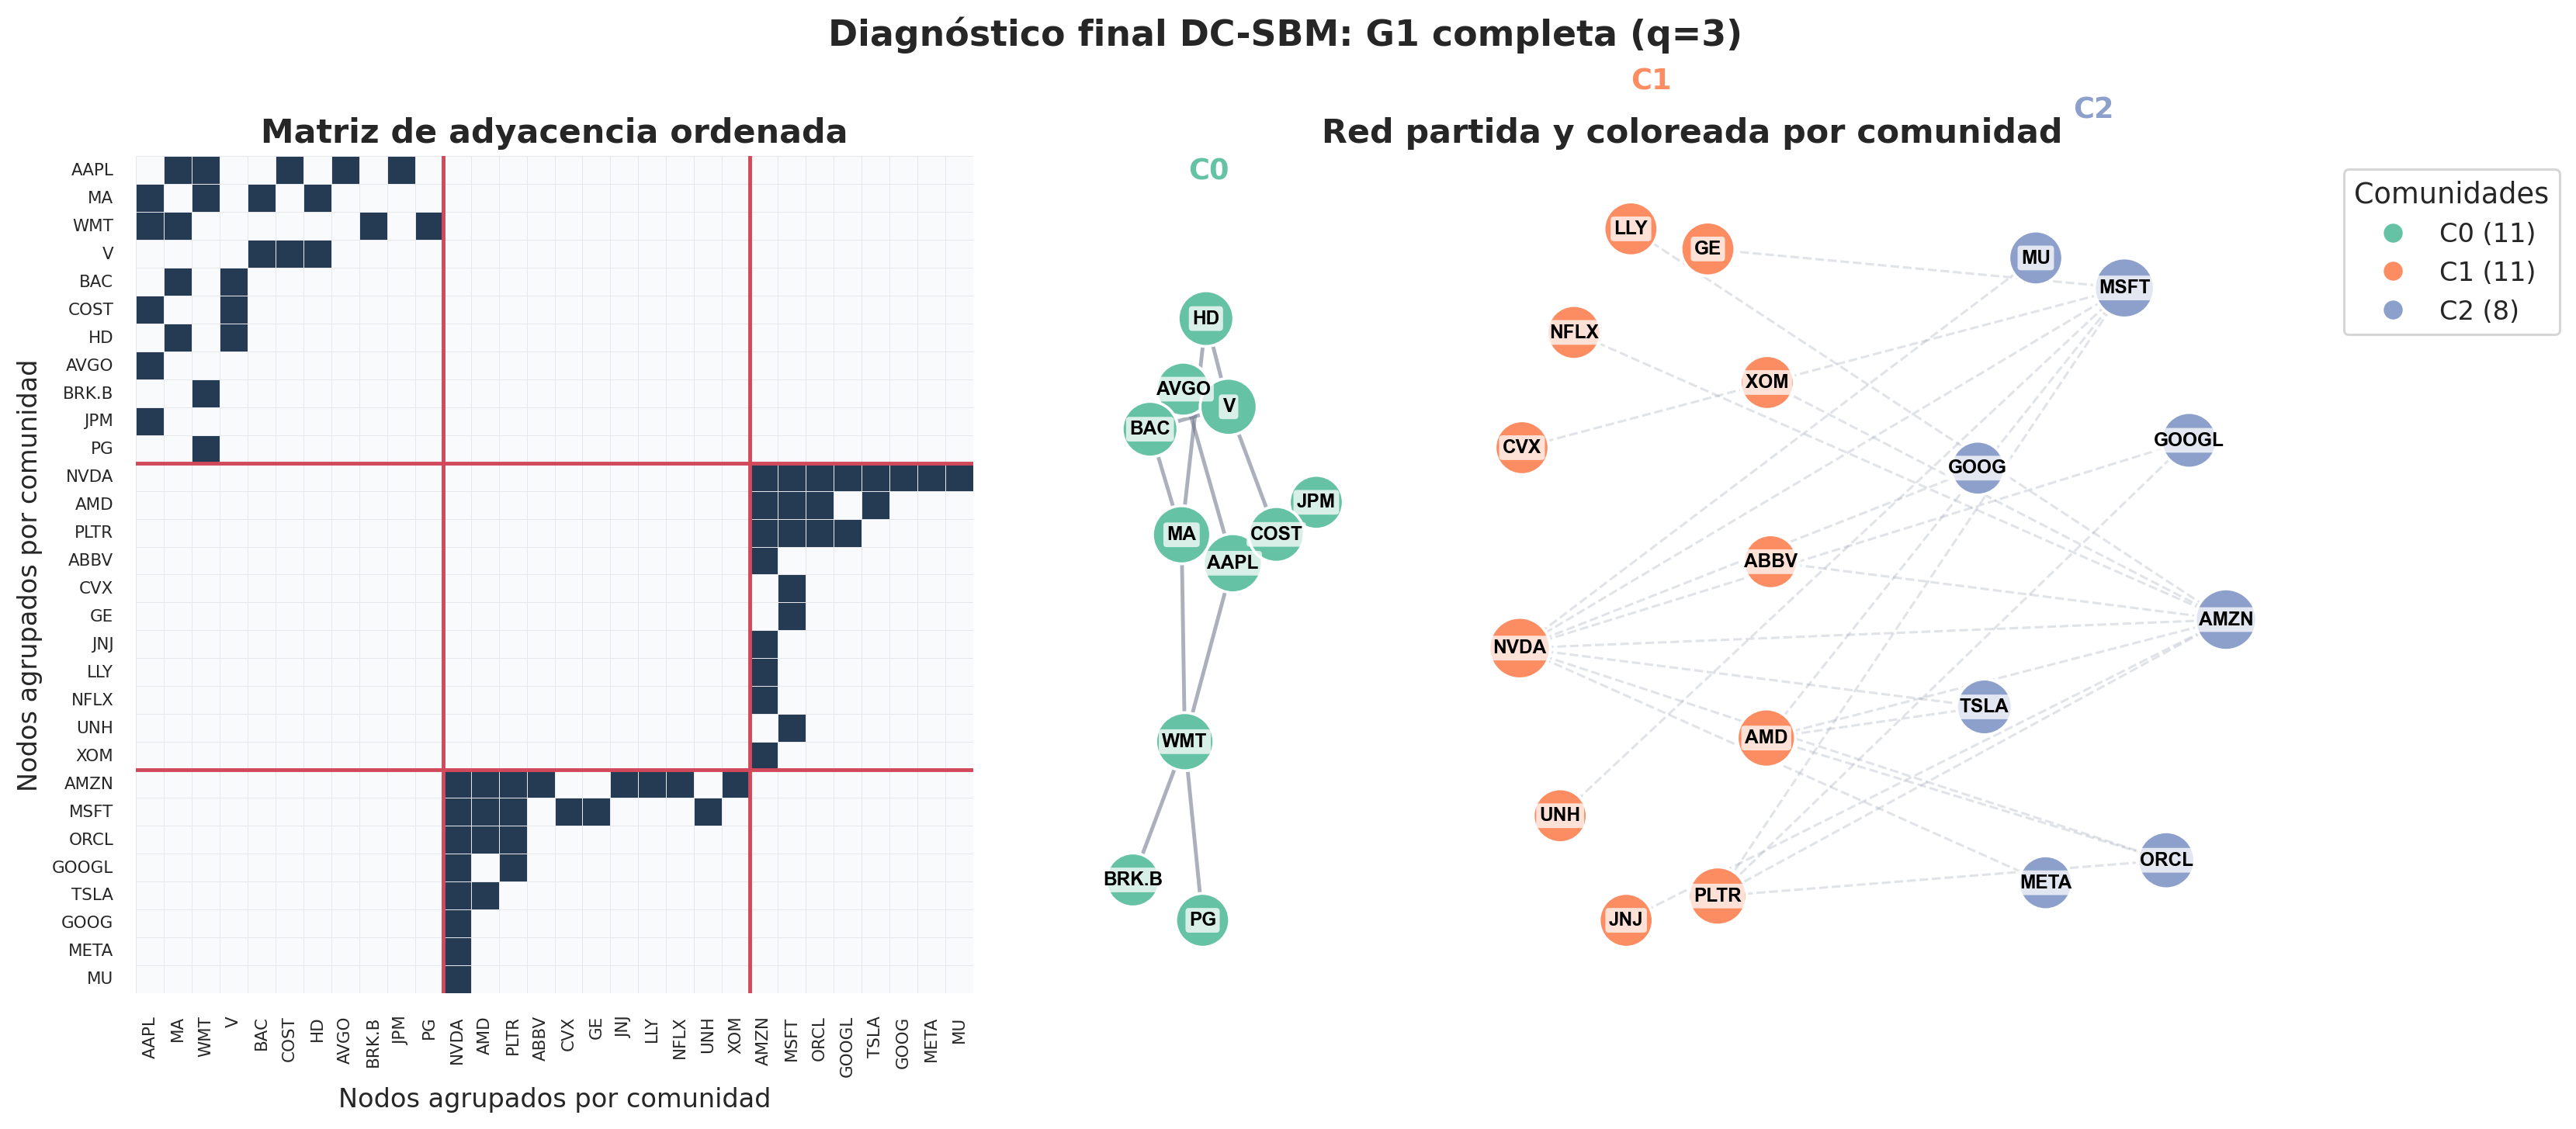
\includegraphics[width=0.95\linewidth]{final_adyacencia_y_red_partida_G1.png}
\caption{Diagnostico final de $G_1$: matriz de adyacencia ordenada y red partida por comunidades.}
\end{figure}

El patron visual confirma la interpretacion matematica:
\begin{itemize}
    \item El grupo $1$ tiene un bloque diagonal, por lo que es asortativo.
    \item Los grupos $2$ y $3$ no tienen bloques diagonales relevantes; sus aristas aparecen fuera de la diagonal.
    \item La baja modularidad diagnostica para $q=3$ no invalida la particion: simplemente indica que la estructura no es puramente modular/asortativa.
\end{itemize}

\section{Explicacion matematica de por que ocurre}

El mecanismo puede verse directamente en la log-verosimilitud perfilada:
\[
    L(g)
    =
    \frac{1}{2}\sum_{r,s}
    m_{rs}\log\left(\frac{m_{rs}}{\kappa_r\kappa_s}\right)
    +\text{constantes}.
\]
Para una particion dada, los pares $(r,s)$ con $m_{rs}=0$ no aportan al sumatorio. Por tanto, el modelo recompensa particiones que concentran la masa observada en pocos pares de bloques, siempre que esa concentracion sea grande en relacion con $\kappa_r\kappa_s$.

En $G_1$ se observan dos concentraciones extremas:
\[
    m_{11}=26,
    \qquad
    m_{23}=m_{32}=24,
\]
y los demas pares son cero. Esto genera una matriz $\hat\Omega$ con solo dos intensidades positivas relevantes. La primera, $\hat\omega_{11}$, explica la comunidad cerrada de consumo/pagos. La segunda, $\hat\omega_{23}$, explica la estructura de roles tecnologicos.

La correccion por grado es crucial. `NVDA', `AMZN' y `MSFT' tienen grados altos, pero el modelo no los agrupa solamente por ser nodos centrales. Primero fija
\[
    \hat c_i=k_i.
\]
Despues pregunta si, dadas esas propensiones individuales, las aristas caen preferentemente dentro de algun grupo o entre ciertos grupos. La respuesta es:
\begin{enumerate}
    \item En consumo/pagos, las aristas caen dentro del mismo grupo.
    \item En tecnologia, las aristas caen entre dos grupos distintos.
\end{enumerate}

Por eso el resultado sustantivo no es ``hay tres comunidades densas''. El resultado correcto es:
\[
    \text{una comunidad asortativa}
    \quad+\quad
    \text{dos roles tecnologicos disasortativos}.
\]

\section{Conclusion}

El DC-SBM muestra que la red no tiene una unica forma de organizacion. Una parte se comporta como comunidad tradicional: el bloque de pagos, retail y consumo tiene conexiones internas y queda separado de la componente tecnologica. Otra parte se comporta como estructura de roles: los nodos tecnologicos se dividen en dos lados con muchas aristas cruzadas y sin aristas internas dentro de cada lado.

La minired confirma esta lectura. Al eliminar nodos de grado $1$, el bloque de consumo/pagos permanece y el cruce plataformas--infraestructura/IA se vuelve aun mas intenso en terminos de $\hat\omega_{rs}$. Por tanto, el valor $q=3$ no es solo una decision numerica del BIC-like; corresponde a una interpretacion estructural clara:
\[
    \boxed{
    \text{pagos/retail}
    \quad\oplus\quad
    \text{plataformas tecnologicas}
    \quad\leftrightarrow\quad
    \text{infraestructura/IA}
    }.
\]

\end{document}
